\documentclass[a4paper]{ctexrep}
\usepackage{ctex}
\usepackage{times}
\usepackage{setspace}
\usepackage{fancyhdr}
\usepackage{graphicx}
\usepackage{wrapfig}
\usepackage{array}  
\usepackage{fontspec,xunicode,xltxtra}
\usepackage{titlesec}
\usepackage{titletoc}
\usepackage[titletoc]{appendix}
\usepackage[top=30mm,bottom=30mm,left=20mm,right=20mm]{geometry}
\usepackage{listings}
\usepackage{enumerate}
\usepackage{algorithm}
\usepackage{algorithmicx}
\usepackage{algpseudocode}

\setmainfont{TeX Gyre Pagella}
\floatname{algorithm}{伪代码}
\renewcommand{\algorithmicrequire}{\textbf{Input:}}
\renewcommand{\algorithmicensure}{\textbf{Output:}}

%---------------------------------------------------------------------
%	页眉页脚设置
%---------------------------------------------------------------------
\fancypagestyle{plain}{
	\pagestyle{fancy}      %改变章节首页页眉
}

\pagestyle{fancy}
\lhead{\kaishu~TCP/IP课程实验报告~}
\rhead{\kaishu~1030616134~尹达恒~}
\cfoot{\thepage}

%---------------------------------------------------------------------
%	章节标题设置
%---------------------------------------------------------------------
\titleformat{\chapter}{\centering\zihao{-1}\heiti}{实验四}{1em}{}
\titlespacing{\chapter}{0pt}{*0}{*6}

%---------------------------------------------------------------------
%	目录页设置
%---------------------------------------------------------------------
\titlecontents{chapter}[0em]{\songti\zihao{-4}}{\thecontentslabel\ }{}
{\hspace{.5em}\titlerule*[4pt]{$\cdot$}\contentspage}
\titlecontents{section}[2em]{\vspace{0.1\baselineskip}\songti\zihao{-4}}{\thecontentslabel\ }{}
{\hspace{.5em}\titlerule*[4pt]{$\cdot$}\contentspage}
\titlecontents{subsection}[4em]{\vspace{0.1\baselineskip}\songti\zihao{-4}}{\thecontentslabel\ }{}
{\hspace{.5em}\titlerule*[4pt]{$\cdot$}\contentspage}

\ctexset {
	chapter = {
		name = {实验},
		number = {四},
	},
	section = {
		number = \arabic{section},
		format = \Large\bfseries,
	},
	subsection = {
		number = \arabic{section}.\arabic{subsection},
	}
}

\begin{document}
%---------------------------------------------------------------------
%	封面设置
%---------------------------------------------------------------------
\begin{titlepage}
	\begin{center}
    
\includegraphics[width=0.9\textwidth]{figure//Njust.png}\\
    \vspace{10mm}
    \textbf{\zihao{2}\kaishu{ 物联网工程学院}}\\[0.8cm]
    \textbf{\zihao{2}\kaishu{ TCP/IP课程实验报告}}\\[3cm]
	\vspace{\fill}
	\setlength{\extrarowheight}{3mm}
	{\songti\zihao{3}	
		\begin{tabular}{rl}
			
			{\makebox[4\ccwd][s]{班\qquad 级:}}& ~\kaishu 物联1601\\
			
			{\makebox[4\ccwd][s]{姓\qquad 名:}}& ~\kaishu 尹达恒 \\ 
			
			{\makebox[4\ccwd][s]{学\qquad 号:}}& ~\kaishu 1030616134 \\ 
			
			{\makebox[4\ccwd][s]{指导老师:}} & ~\kaishu 马君霞\\ 
			
		\end{tabular}
	}\\[2cm]
	\vspace{\fill}
	\zihao{4}
	2018\textasciitilde 2019第一学期\\
	\today
	\end{center}	
\end{titlepage}



%---------------------------------------------------------------------
%  目录页
%---------------------------------------------------------------------
\tableofcontents % 生成目录
%---------------------------------------------------------------------
%  实验一
%---------------------------------------------------------------------
\chapter{基于TCP协议的客户端/服务器回声程序}
\begin{spacing}{1.5}
\songti\zihao{-4}
\section{实验目的及要求}
\begin{itemize}
	\item 了解和掌握“基于TCP 连接的应用程序”的运行机制和编程方法;
	\item 编写一个基于TCP协议的客户/服务器回声程序;
	\item 掌握从命令行连续输入信息并进行发送的编程方法。
\end{itemize}
\section{实验环境}
\begin{itemize}
	\item 操作环境:Windows 10;
	\item 编程环境:Visual Studio 2015;
	\item 程序使用Visual Studio下的控制台程序“Win32 Console Application”。
\end{itemize}
\section{实验内容及步骤}
\subsection{服务器端程序}
该程序中通信协议使用的是面向连接的提出TCP协议(SOCK\_STREAM)。服务器端的IP地址使用系统指定的IP地址,端口号在程序中指定为5555,用符号常量来定义。
\begin{itemize}
	\item 调试环境:Visual Stdio 2015
	\item 服务器IP地址:由系统指定
	\item 服务器端口号:5050
	\item 程序名称:TCPserver.cpp
	\item 程序功能:服务器端的程序当有客户提出连接请求时,在端口5050与客户端进行TCP连接,连接成功后,把从客户端收到的信息原样转发给客户端程序,并显示接收到的数据和所发送的字节数。当收到字符“0”时退出
	\item 程序伪代码:伪代码\ref{serverprog}
	\begin{algorithm}[h]
		\caption{服务器端程序}\label{serverprog}
		\begin{algorithmic}[1]
			\State 变量初始化
			\State WSAStartup()启动winsocket
			\State socket()建立流式套接字
			\State bind()将流式套接字与服务器地址和端口绑定
			\State listen()开始监听
			\State accept()等待接收连接请求
			\State 与客户端建立连接
			\Ensure 显示客户端地址和端口号
			\Repeat
			\State recv()接收客户端数据
			\Ensure 显示接收到的数据
			\State send()将接收到的数据发回客户端
			\Ensure 显示发回客户端的字节数
			\Until{接收到的数据是字符“0”}
			\State closesocket()关闭和客户端的连接
			\State closesocket()关闭服务器端流式套接字
			\State WSACleanup()关闭winsocket
			\State 退出程序
		\end{algorithmic}
	\end{algorithm}
\end{itemize}
\subsection{客户端程序}
\begin{itemize}
	\item 调试环境:Visual Stdio 2015
	\item 客户IP地址和端口:由系统指定
	\item 程序名称:TCPclient.cpp
	\item 程序功能:客户端程序向服务器提出TCP连接的请求,当连接建立后,从服务器的端口5050接收数据,连续多次向服务器发送信息,并显示从服务器收到的信息。
	\item 命令格式:点分十进制形式的服务器IP地址
	\item 命令举例:192.168.137.1
	\item 程序伪代码:伪代码\ref{clientprog}
	\begin{algorithm}[h]
		\caption{客户端程序}\label{clientprog}
		\begin{algorithmic}[1]
			\State 变量初始化
			\State WSAStartup()启动winsocket
			\State socket()建立流式套接字
			\Require 输入服务器IP地址
			\State connect()向输入的IP地址发起连接
			\Repeat
			\Require 输入要发送的数据
			\State send()将输入的数据发向服务器端
			\State recv()接收服务器发回的数据
			\Ensure 显示从服务器发回的数据
			\Until{发送的数据是字符“0”}
			\State closesocket()关闭和服务器端的连接
			\State WSACleanup()关闭winsocket
			\State 退出程序
		\end{algorithmic}
	\end{algorithm}
\end{itemize}
\newpage
\subsection{本机回环测试}
\begin{itemize}
	\item 测试环境:Visual Studio 2015
	\item 测试步骤:
	\begin{enumerate}
		\item 在同一台主机上同时启动服务器和客户端程序;
		\item 在客户端程序中输入IP地址“127.0.0.1”进行连接;
		\item 在客户端中依次输入并发送“How”、“are”、“you”、“0”;
		\item 观察记录控制台输出。
	\end{enumerate}
\end{itemize}

\subsection{远程互通测试}
\begin{itemize}
	\item 测试环境:Visual Studio 2015
	\item 测试步骤:
	\begin{enumerate}
		\item 将两台主机连入同一个网络;
		\item 分别在两台主机上的命令行窗口输入命令“ipconfig”查看并记录各自的IP地址;
		\item 在一台主机上启动服务器程序,另一台主机上启动客户端程序;
		\item 在客户端程序中输入服务器端主机的IP地址进行连接;
		\item 在客户端中依次输入并发送“How”、“are”、“you”、“0”;
		\item 观察记录控制台输出;
		\item 交换运行两台主机的服务器和客户端程序并重复步骤3至步骤6。
	\end{enumerate}
\end{itemize}

\section{实验结果}
\subsection{本地回环测试结果}
服务器端:图\ref{localserver}
\begin{figure}[htbp]
	\centering
	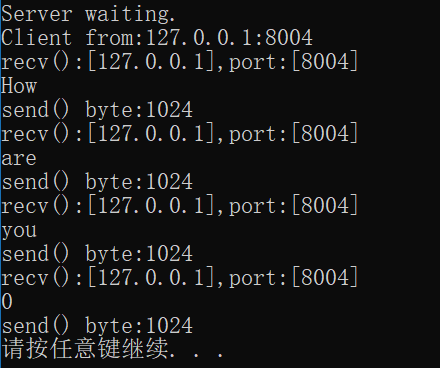
\includegraphics [width=0.5\textwidth]{figure//localserver.png}
	\caption{本地回环服务器端测试结果}\label{localserver}
\end{figure}

客户端:图\ref{localclient}
\begin{figure}[htbp]
	\centering
	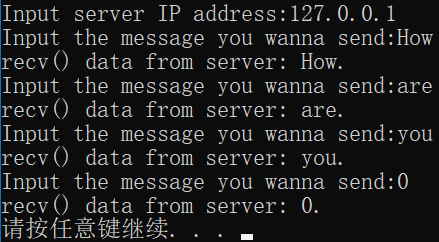
\includegraphics [width=0.5\textwidth]{figure//localclient.png}
	\caption{本地回环客户端测试结果}\label{localclient}
\end{figure}

\newpage
\subsection{远程互通IP记录}
主机1:图\ref{IP1}
\begin{figure}[htbp]
	\centering
	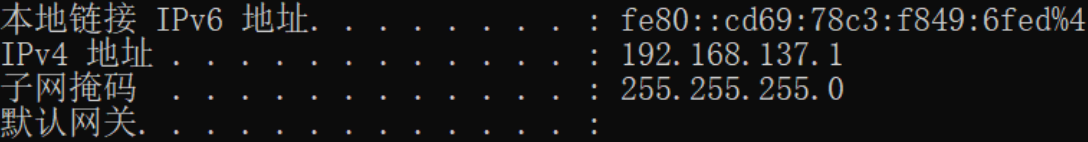
\includegraphics [width=1\textwidth]{figure//IP1.png}
	\caption{主机1IP}\label{IP1}
\end{figure}

主机2:图\ref{IP2}
\begin{figure}[htbp]
	\centering
	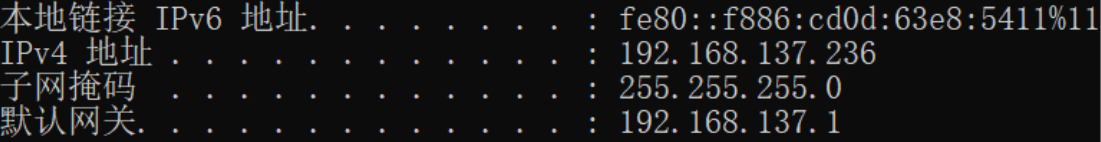
\includegraphics [width=1\textwidth]{figure//IP2.png}
	\caption{主机2IP}\label{IP2}
\end{figure}

\subsection{远程互通测试1结果(主机A做服务器端,主机B做客户端)}
主机1:图\ref{remote1local1}
\begin{figure}[htbp]
	\centering
	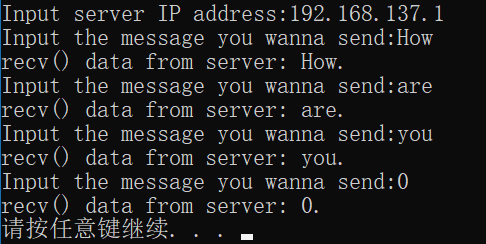
\includegraphics [width=0.5\textwidth]{figure//remote1local2.png}
	\caption{远程互通测试2主机2结果}\label{remote1local1}
\end{figure}

\newpage
主机2:图\ref{remote1local2}
\begin{figure}[htbp]
	\centering
	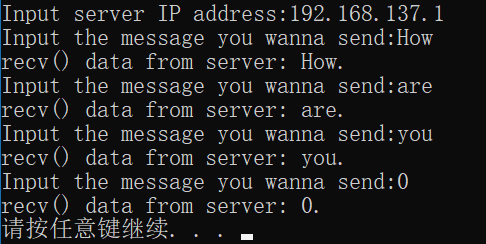
\includegraphics [width=0.5\textwidth]{figure//remote1local2.png}
	\caption{远程互通测试1主机1结果}\label{remote1local2}
\end{figure}

\subsection{远程互通测试2结果(主机A做客户端,主机B做服务器端)}
主机1:图\ref{remote2local1}
\begin{figure}[htbp]
	\centering
	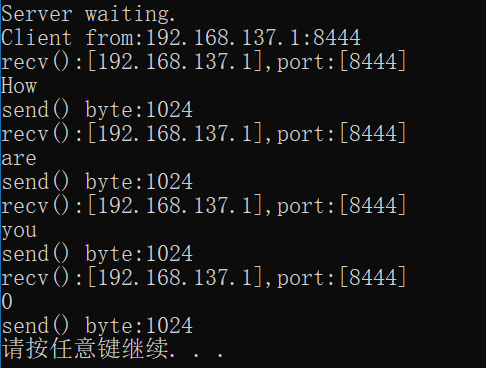
\includegraphics [width=0.5\textwidth]{figure//remote2local2.png}
	\caption{远程互通测试2主机1结果}\label{remote2local1}
\end{figure}

\newpage
主机2:图\ref{remote2local2}
\begin{figure}[htbp]
	\centering
	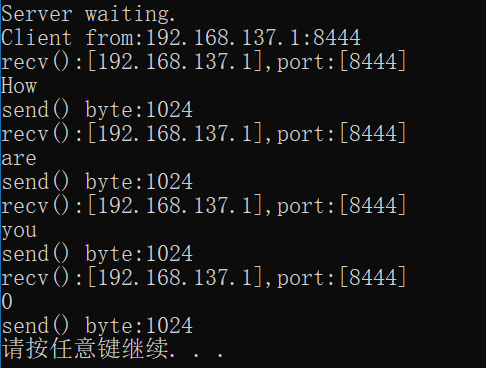
\includegraphics [width=0.5\textwidth]{figure//remote2local2.png}
	\caption{远程互通测试2主机2结果}\label{remote2local2}
\end{figure}

\end{spacing}
\section{问题及心得}
	\begin{itemize}
		\item 问题:经过前几次实验的积累,本次实验的程序为在实验一的代码基础上进行修改而来,实验非常顺利,没有遇到阻碍实验进行的问题。
		\item 心得:\begin{enumerate}
			\item 实践是检验真理的唯一标准;
			\item 实验是巩固知识的最快捷径;
			\item 更加深入地理解了TCP协议的运行过程;
			\item 明白了winsocket程序开发的一般模式;
			\item 精进了代码水平。
		\end{enumerate}
	\end{itemize}
\end{document}